\chapter{}

用多种(至少两个)方法求解差分方程:
\begin{equation*}
    \begin{split}
        &2x_{n+2} - x_{n+1} - 2x_n = 0\\
        &x_0 = -2\\
        &x_1 = 0
    \end{split}
\end{equation*}
\section{方法一:特征方程法}
此题为齐次线性差分方程。

特征方程为

\begin{equation}
    2\lambda^2-\lambda-2=0
\end{equation}

解得方程的解为

$\lambda_1 = \dfrac{1+\sqrt[]{17}}{4}, \lambda_2 = \dfrac{1-\sqrt[]{17}}{4} $

则$x_n=c_1\lambda_1^n + c_2\lambda_2^n = c_1(\dfrac{1+\sqrt[]{17}}{4})^n + c_2(\dfrac{1-\sqrt[]{17}}{4})^n$


带入初始条件得:

\begin{equation}
    \begin{aligned}
        &c_1+c_2=-2\\
        &\dfrac{1+\sqrt[]{17}}{4}c_1 + \dfrac{1-\sqrt[]{17}}{4}c_2 = 0
    \end{aligned}
\end{equation}

得$c_1=-1+\frac{\sqrt[]{17}}{17}, c_2=-1-\frac{\sqrt[]{17}}{17}$

因此有$x_n = (-1+\dfrac{\sqrt[]{17}}{17})(\dfrac{1+\sqrt[]{17}}{4})^n+(-1-\dfrac{\sqrt[]{17}}{17})( \dfrac{1-\sqrt[]{17}}{4} )^n$


\section{方法二:线性代数法}

将方程进行等价变形,得

\begin{equation}
    \left \{
        \begin{aligned}
        &x_{n+2} = \frac{1}{2}x_{n+1} + x_n\\
        &x_{n+1} = x_{n+1}
        \end{aligned}
    \right .
\end{equation}

因此有转移矩阵方程

\begin{equation}
    \begin{bmatrix}
        x_{n+2} \\
        x_{n+1} 
    \end{bmatrix} =
    \begin{bmatrix}
        \frac{1}{2} & 1 \\
        1 & 0 
    \end{bmatrix}
    \begin{bmatrix}
        x_{n+1} \\
        x_n
    \end{bmatrix}
\end{equation}

设$A = \begin{bmatrix}
    \frac{1}{2} & 1 \\
    1 & 0 
\end{bmatrix}$,则有

\begin{equation}
    \begin{bmatrix}
        x_{n+1} \\
        x_{n} 
    \end{bmatrix} =
    A^n
    \begin{bmatrix}
        x_{1} \\
        x_0
    \end{bmatrix}
\end{equation}

矩阵$A$的特征方程为

\begin{equation}
    \begin{split}  
   |\lambda E - A | &= 
   \begin{vmatrix}
    \lambda - \frac{1}{2} & -1 \\
    -1 & \lambda 
   \end{vmatrix}
   \\
   &=(\lambda -\frac{1}{2})\lambda - 1\\
   &= \lambda ^ 2 - \frac{1}{2} \lambda  -1
\end{split}
\end{equation}

得$\lambda_{1,2} = \frac{1 \pm \sqrt{17} }{4} $

将矩阵相似对角化得

\begin{equation}
    \begin{aligned}
    &A = PDP^{-1} \\
    &P = \begin{bmatrix}
        \dfrac{1-\sqrt[]{17}}{4} & \dfrac{1+\sqrt[]{17}}{4} \\
        1 & 1 
    \end{bmatrix}
    \\
    &D=\begin{bmatrix}
        \dfrac{1-\sqrt[]{17}}{4} & 0 \\
        0 & \dfrac{1+\sqrt[]{17}}{4} 
    \end{bmatrix}
\end{aligned} 
\end{equation}

因此最终解得

\begin{equation}
    \begin{aligned}
    \begin{bmatrix}
        x_{n+1} \\
        x_{n} 
    \end{bmatrix} &= 
    A^n
    \begin{bmatrix}
        x_{1} \\
        x_0
    \end{bmatrix}\\
     &= PD^nP^{-1}\begin{bmatrix}
        x_{1} \\
        x_0
    \end{bmatrix}\\
    &= \begin{bmatrix}
        \dfrac{(-1 + \sqrt[]{17})(\frac{1-\sqrt[]{17}}{4})^n}{\frac{17-\sqrt[]{17}}{4}} - (\frac{1+\sqrt[]{17}}{2})(\frac{17-\sqrt[]{17}}{34})(\frac{1+\sqrt[]{17}}{4})^n \\
        (-1+\frac{\sqrt[]{17}}{17})(\frac{1+\sqrt[]{17}}{4})^n+(-1-\frac{\sqrt[]{17}}{17})( \frac{1-\sqrt[]{17}}{4} )^n
    \end{bmatrix}
\end{aligned}
\end{equation}

因此有$x_n = (-1+\frac{\sqrt[]{17}}{17})(\frac{1+\sqrt[]{17}}{4})^n+(-1-\frac{\sqrt[]{17}}{17})( \frac{1-\sqrt[]{17}}{4} )^n$

\chapter{}


求下列微分方程的解析解和数值解,并画出曲线图,曲线图范围$t\in[0,1]$。
\begin{equation*}
    \left \{
        \begin{aligned}
            &\frac{\partial x}{\partial t} = x - 2y\\
            &\frac{\partial y}{\partial t} = x + 2y\\
            &x(0)=1, y(0) = 0
        \end{aligned}
    \right . 
\end{equation*}

\section{解析解}

利用sympy库,求解微分方程组,得到的解析解如下。

\begin{equation}
    \begin{aligned}
        x(t) &=\dfrac{-\sqrt[]{7}e^{\frac{3t}{2}}sin(\frac{\sqrt[]{7}t}{2})}{7} + e^{\frac{3t}{2}}cos(\frac{\sqrt[]{7}t}{2})\\
        y(t) &= \dfrac{2\sqrt{7}e^{\frac{3t}{2}}sin(\frac{\sqrt[]{7}t}{2})}{7}
    \end{aligned}
\end{equation}

\section{数值解}

此方程组是一阶常微分方程组,直接利用 scipy.integrate 模块的 odeint 函数求解,并用pylab作图。
x-t图如\ref{fig:x-t},y-t图如\ref{fig:y-t},y-x图如\ref{fig:y-x}。

\begin{figure}[htbp]
    \begin{center}
        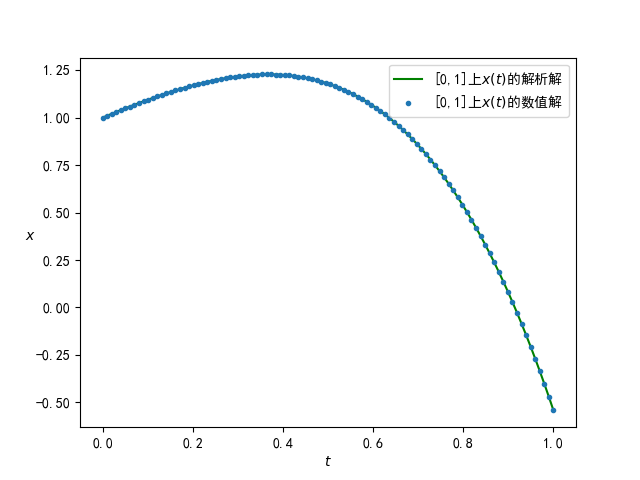
\includegraphics[width=0.9\textwidth]{x-t.png}
    \end{center}
   \caption[]{$x-t$}
    \label{fig:x-t}
\end{figure}

\begin{figure}[htbp]
    \begin{center}
        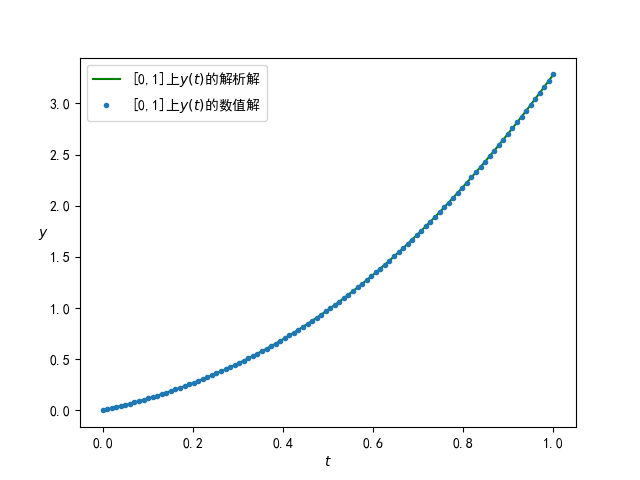
\includegraphics[width=0.9\textwidth]{y-t.png}
    \end{center}
   \caption[]{$y-t$}
    \label{fig:y-t}
\end{figure}

\begin{figure}[htbp]
    \begin{center}
        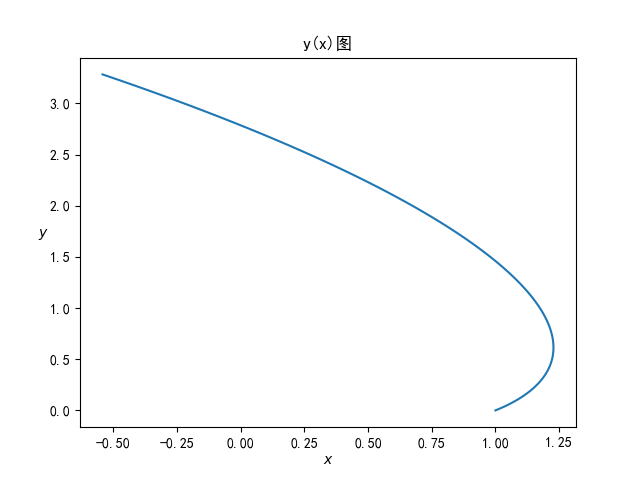
\includegraphics[width=0.9\textwidth]{y-x.png}
    \end{center}
   \caption[]{$y-x$}
    \label{fig:y-x}
\end{figure}